\documentclass[12pt,a4,twoside]{article}

\usepackage[english]{babel}
\usepackage{graphicx}
\usepackage{color}
\usepackage{cite}
\usepackage[mathcal]{eucal}
\usepackage{amsmath}
\usepackage{footnote}
\usepackage{multirow}
\usepackage{eurosym}
\usepackage{url}
\usepackage{hyperref}
% Normal DIN A4 page format
%
\setlength{\marginparwidth}{0cm}
%%\setlength{\evensidemargin}{0cm}
%\setlength{\textheight}{23cm}
%\setlength{\textwidth}{17.5cm}
%%\setlength{\marginparwidth}{-2cm}
\setlength{\evensidemargin}{0cm}
\setlength{\oddsidemargin}{0cm}
%\setlength{\voffset}{-2cm}
\setlength{\hoffset}{-0.5cm}
\textheight 20.5cm
\textwidth 17.0cm
\oddsidemargin 10pt
\evensidemargin 10pt
\setlength{\topmargin}{0.0cm}
\addtolength{\topmargin}{-30pt}
\addtolength{\textheight}{60pt}
%distance between paragraphs
\setlength{\parindent}{0.0em}
\setlength{\parskip}{5pt plus 2pt minus 1pt}
%%%%%%%%%%%%%% To give more room to figures %%%%%%%%%%%%%%%%%%%%%%%
\setcounter{topnumber}{9}
\setcounter{bottomnumber}{9}
\setcounter{totalnumber}{9}
\renewcommand{\textfraction}{0.0}
\renewcommand{\topfraction}{1.0}
\renewcommand{\bottomfraction}{1.0}
%%%%%%%%%%%%%%%%%%%%%%%%%%%%%%%%%%%%%%%%%%%%%%%%%%%%%%%%%%%%%
\frenchspacing
\sloppy
%%%%%%%%%%%%%%%%%%%%%%%% Page Headings %%%%%%%%%%%%%%%%%%%%%%%%%%%%%%
\usepackage{fancyhdr}
\pagestyle{fancy}
%\rhead{Dr. V. Boccone}
%\lfoot{\thepage}
%\rfoot{\thepage}
\usepackage{lastpage}
\cfoot{\thepage\ of \pageref{LastPage}}

\makeatletter
\renewcommand{\@maketitle}{
\newpage
 \null
 \vskip 2em%
  {\LARGE \bf \@title \par}%
  {\@author \par}
 \par} \makeatother

 
 

\def\mul{\multicolumn}
\def\dyfr{\D\frac}
\def\mysection#1{\section{#1}\label{sec: #1}}
\def\mysubsection#1{\subsection{#1}\label{subsec: #1}}
\def\mysubsubsection#1{\subsubsection{#1}\label{subsubsec: #1}}
\def\mysubsubsubsection#1{\paragraph{#1}\label{subsubsubsec: #1}{~}}
\setcounter{secnumdepth}{5}
\def\version{v0.1 Draft}

\begin{document} 
\title{FACT Shutter User Guide - \version}
\author{V.~Boccone} % Dr.
\maketitle 
%\vspace*{0 mm}
%\address{D\'epartement de physique nucl\'eaire et corpusculaire (DPNC),
% 24, Quai Ernest-Ansermet \\
%1211 Gen\'eve \\
%{\rm E-mail: boccone@cern.ch}}
\vspace*{-54mm}
\begin{figure}[h]
\includegraphics[width=40mm]{unigeLogo.jpg}
\end{figure}
\vspace*{-28mm}
{\flushright 
\hfill{\bf FACT Shutter (ab)User Guide - \version}\\
\hfill{\today}\\
\hfill{boccone@cern.ch}}
\vspace*{40 mm}

\section{\label{sec:1} System overview}
The new remotely controllable shutter system for the FACT telescope is built around two LA23 low voltage 24~V linear actuators from Linak\footnote{Linak AG} driven by two VHN-5019 motor driver which are controlled by an Arduino Ethernet micro controller board.

The two linear actuators are fixed on a modified of the T-shaped cable support plates and on a L-shaped support which is shrewd to the lid. The T and L-shaped supports are made in blue anodized aluminum and are shown in Fig.\ref{figShutterPhoto}.

\begin{figure}[b!]
\centering
\includegraphics[width=0.49\textwidth]{shutter_photo1.jpg}
\includegraphics[width=0.49\textwidth]{shutter_photo2.jpg}
\caption{\label{figShutterPhoto} {Photograph of the installed shutter motor}}
\end{figure}

The Arduino is an open-source electronics prototyping platform based on the ATmega AVR micro-controller line. We chose the {\bf Arduino Ethernet} model which mounts a ATmega328 micro-controller with has 32 KB of ROM  and 2 KB of SRAM and it already includes a 10 Mbit ethernet interface using a WizNet W5100 chipset.

The Arduino boards feature a bus like structure on the sides where composed by two lines of pass through connectors where  Arduino compatible boars (shields) can be plugged in. Arduino shields are normally stackable
and more shields can be mounted on one controller, provided that their pinout are compatibles.
\begin{figure}[b!]
\centering
\includegraphics[width=1\textwidth]{shutter_sketch.pdf}
\caption{\label{figShutterSketch} {Sketch of the shutter system}}
\end{figure}

A sketch of the new shutter system is shown in Fig.\ref{figShutterSketch}. The two motors are connected to an Arduino\cite{arduino} shield which contains two VHN-5019 motor drivers which also enable current sensing. A filter/amplifier shield has been developed to reduce the noise  on the position sensor and on the current measurement which is mainly caused by the length of the cables to the telescope (about 35 m).

The firmware can be uploaded in the Arduino through a standard RS232 serial port although an USB to Serial converter adapter is provided with the board. The firmware which is currently uploaded provide a simple web server with two button linked to the opening and closing commands of the shutter.

\subsection{The motor controller shield}
The motor controller shield is a {\bf Pololu Dual VNH5019 Motor Driver Shield\footnote{\href{http://www.pololu.com/catalog/product/2502}{http://www.pololu.com/catalog/product/2502}}}. The schematic of the shield and the layout of the connection are shown in Fig.\ref{figMotorShield} and Fig.\ref{figMotorShieldUse} respectively.
\begin{figure}[b!]
\centering
\includegraphics[width=0.77\textwidth]{pololu_sch_small.png}
\caption{\label{figMotorShield} {Diagram of the dual VHN5019 motor driver Arduino shield}}
\end{figure}

Each of the VHN-5019 is able to control - with few external components - a mid-high power motor using continuous current or Pulse Width Modulation (PWM) and - in addition - grants the possibility of performing the motor current sensing using the A0 ({\bf M1CS} signal) and A1 ({\bf M2CS} signal) Arduino analog inputs by embedding on the chip a current to voltage converter with a current sensing coefficient of 0.14 V/A. 

Other then the A0 and A1 Arduino analog inputs the shield uses three additional digital I/O Arduino ports for each motors.
The {\bf MxINA} and {\bf MxINB} signals, connected to pins 2/3 for motor 1 and pins 7/8 for motor 2, define the status of each motor (on/off) while the {\bf MxPWM} signals, connected to pins 5 and 6 for motor 1 and motor 2 respectively, define the speed.

The motors together with the main motor power supply (24~V) are connected to the front 6-ways connector as indicated in the Fig.\ref{figMotorShieldUse}. 
%In view of an - almost - completely remote operability of the FACT telescope the shutter
%The new system was adapted as much as possible on the old mechanics.... 
%Each lid can move independently by a 55 mm stroke actuator which grant the necessary excursion to reach the $110^{\circ}$ which is required in order no to shadow the camera.

\begin{figure}[t!]
\centering
\includegraphics[width=0.6\textwidth]{pololu_use.jpg}
\caption{\label{figMotorShieldUse} {Connection layout of the dual VHN5019 motor driver Arduino shield}}
\end{figure}
\subsection{Amplifier and filter shield}
The system is completed by a amplifier and filter shield which has the double task of:\begin{itemize}
\item reducing the noise of the hall sensors accumulated over the 35 m of cables with a low-pass filter \mbox{($\nu_{\rm Low~Cut}=1~$ kHz)};
\item producing a second low current sensing measurement on pin A4 and A5 by amplifying ($\times 10$) and filtering \mbox{($\nu_{\rm Low~Cut}=1~$ kHz)} the signals on the A0 and A1 pins produced by the VHN-5019 chips.
\end{itemize}
The diagram of the filter/amplifier Arduino shield is shown in Fig.\ref{figFilterShield}. The design includes test pins and a set of jumper used for disable the amplification or the filter in case of need.
\begin{figure}[t!]
\centering
\includegraphics[width=1\textwidth]{dpnc303_sch.pdf}
\caption{\label{figFilterShield} {Diagram of the custom filter/amplifier Arduino shield}}
\end{figure}
%In view of low current measurement, two 10x amplifiers followed by each preceded by a low pass 2$^{nd}$ \mbox{($\nu_{cut}=1~$ kHz)} Butterworth filters were included on a custom circuit mounted as an Arduino shield. The diagram of the filter/amplifier Arduino shield is shown in Fig.\ref{figFilterShield}. The input current sensing signal is taken from the A0 and A1 analog Arduino pins while the amplified and filtered output is fed on the A4 and A5 analog pins respectively.
% The analog signals of the Hall position sensors are also fed a low pass 2$^{nd}$ \mbox{($\nu_{cut}=1~$ kHz)} Butterworth filters and their output is connected to the A2/A3 analog Arduino pins.
\subsection{Possible upgrades}
The pin 4 and pin 9 Arduino I/O port were also connected to lemo cable in case - for example - of future wire coupling with other subsystems (i.e. the interlock system)
\clearpage
\section{Cabling and connection}
The LA23 actuators requires 5 electrical connection as shown in Fig.\ref{figLA23connector}:
\begin{itemize}
\item$2\times$ AWG20 wires for the powering of the motor;
\item$3\times$ AWG24 wires for the powering and the output signal of the Hall potentiometer sensor.
\end{itemize}
\begin{figure}[h!]
\centering
\includegraphics[width=0.5\textwidth]{LA23_connector.jpg}
\caption{\label{figLA23connector} {Connection diagram for the Linak LA 23 actuator}}
\end{figure}

The linear actuators are provided by Linak with a custom proprietary cable fitted with sealed connector which contains a total of $8\times$ AWG20/24 wires of which only 5 are used from the LA23 actuators. The maximal cable length is 5~m and the provided cable is not shielded. For this reason we reduced the custom cable length to the minimum (about 70~cm) and we used 35~m of UV-resistent shielded cable instead to reach the control electronics.
%The patch connector is a 
In view on the PWM operation, the unused wires of the actuator cable were connected to ground with the goal of reducing the noise on the Hall potentiometer and current sensing measurement.
\begin{figure}[h!]
\centering
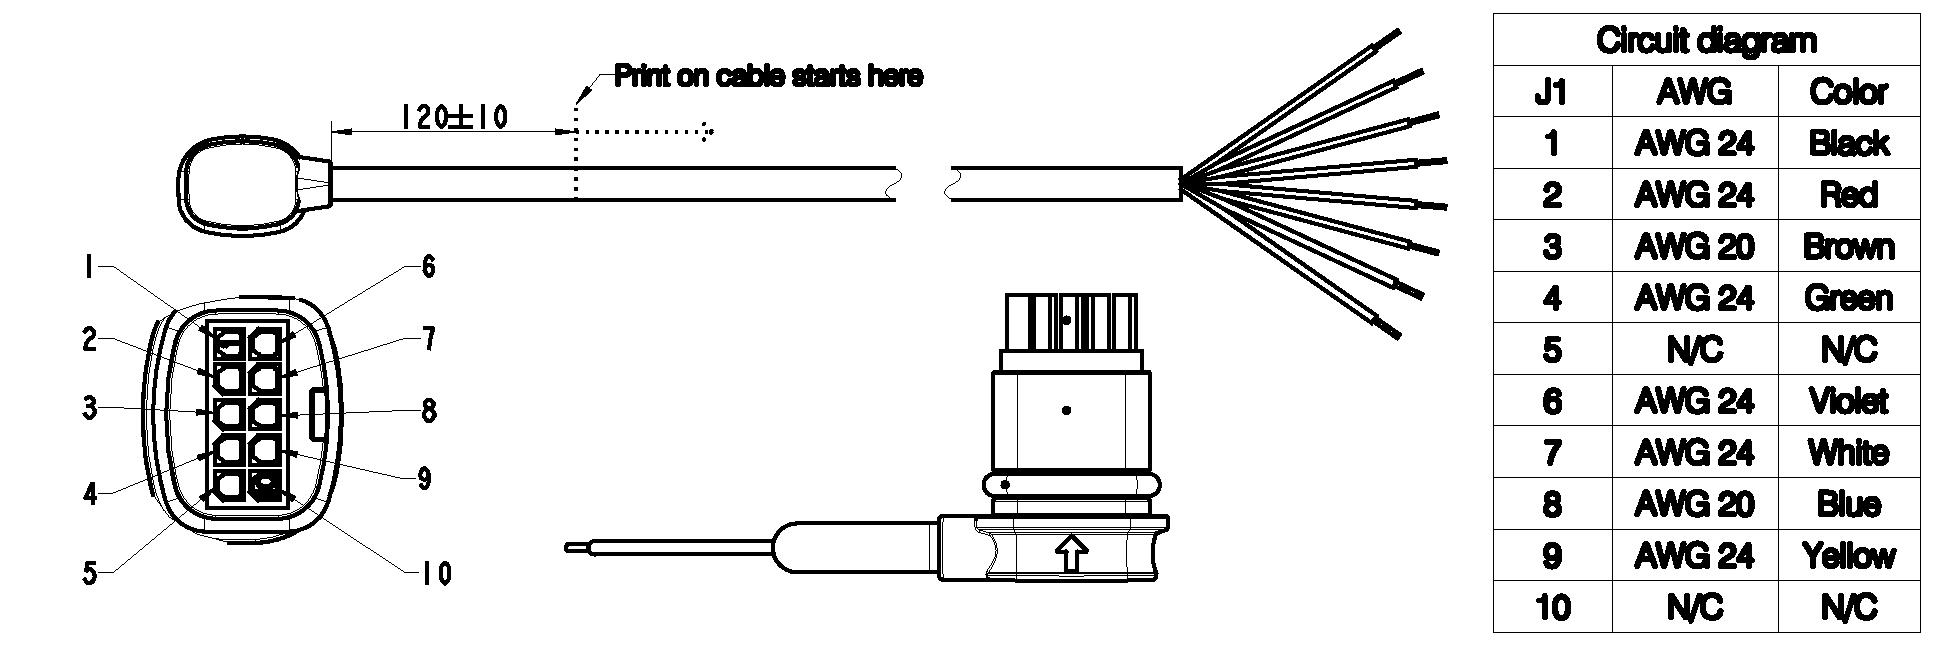
\includegraphics[width=0.9\textwidth]{LA23_cable.pdf}
\caption{\label{figLA23cable} {Cable specifications for the Linak actuators}}
\end{figure}


%\section{Diagram of the filter board}

\section{Functional flow block diagram}
To be completed.

\section{The preliminary web interface}
A web interface to operate the shutter is available at \href{http://10.0.100.36}{http://10.0.100.36} within the fact internal network. [To be completed]

\begin{thebibliography}{50}
\small
\bibitem{arduino} \href{http://www.arduino.cc}{http://www.arduino.cc}
\end{thebibliography}
\end{document}
